\documentclass[11pt]{article}
% EACL Demo is single-blind. Keep ACL review line and page numbers,
% while showing the author block. Do not modify the official style file.
\usepackage[review]{acl}
\makeatletter
\ifdefined\LMDocAnonymous\else\acl@anonymizefalse\fi
\makeatother
\usepackage{times}
\usepackage{latexsym}
\usepackage[T1]{fontenc}
\usepackage[utf8]{inputenc}
\hyphenation{LMDoc}
\usepackage{microtype}
\usepackage{inconsolata}
\usepackage{graphicx}
\usepackage{booktabs}
\usepackage{tabularx}
\usepackage{array}
\usepackage{amsmath}
\usepackage{enumitem}
\usepackage{tikz}
\usepackage{xurl}
\usetikzlibrary{arrows.meta,positioning}
\Urlmuskip=0mu plus 2mu\relax
\setlist[itemize]{leftmargin=*,itemsep=1pt,topsep=2pt}
\setlist[enumerate]{leftmargin=*,itemsep=1pt,topsep=2pt}
\newcommand{\route}[1]{\texttt{#1}}
\author{Chenghao Zhang \quad Ke Xu \quad Xiao Xiao \quad Meng Fang\\
School of Computer Science and Informatics, University of Liverpool}
\title{LMDoc: A Local-First Workbench for Observable Multimodal Document Question Answering}
\hypersetup{pdftitle={LMDoc: A Local-First Workbench for Observable Multimodal Document Question Answering},
pdfauthor={Chenghao Zhang, Ke Xu, Xiao Xiao, Meng Fang}}
\ifdefined\LMDocAnonymous\hypersetup{pdfauthor={Anonymous}}\fi
\begin{document}
\maketitle
\raggedbottom
\begin{abstract}
While retrieval-augmented generation shows promise for grounding language-model outputs, route-aware evidence selection, citation grounding, and abstention for multimodal document collections remain understudied. We introduce MARA on academic and technical document collections spanning text scientific QA, citation-grounded answer generation, and multimodal document QA. We evaluate its answer quality, citation grounding, and route-level behaviour across a full-system benchmark of 41 artifact sets and 3,540 prediction records. Our  model demonstrates efficient performance on text-heavy and citation-grounded tasks, suggesting that route-aware control
preserves competitive answer quality while adding
observability. MARA provides a practical and inspectable environment for privacy-conscious multimodal document analysis. We provide a local-first document QA application allowing users to experience route-aware retrieval and answering firsthand. MARA's document QA capabilities are demonstrated across text, page-image, and hybrid evidence routes, offering valuable insights for researchers and practitioners building transparent, route-aware multimodal document QA systems as alternatives to fixed and text-only retrieval pipelines.

%MARA is a local-first workbench for document question answering over mixed technical and academic collections. It extends a basic local QA framework, inherited from Kotaemon, with a route-aware controller, shared Web and CLI workflows, multimodal evidence routes, citation and trace observability, and a benchmark harness for route-level diagnosis. The main technical feature is a Self-RAG-inspired controller implemented as explicit program decisions rather than as a trained reflection-token model. Given a question and selected sources, the controller inspects text, visual, element, and graph evidence availability; starts from fixed, planner-supplied, or heuristic route decisions; applies heuristic route-scoring proxies when probe evidence is available; selects among text RAG, page-image/VLM, hybrid, guarded retrieval, graph, direct, and abstention behaviours; and returns answer, citation, evidence, workflow-cost, and verification traces. A full-system benchmark over 41 completed artefact sets and 3,540 prediction records shows that MARA's controller behaviour is measurable across text-heavy, citation-based, and multimodal QA settings. The paper presents the approach, experiments and results, demonstration use case, related work, and the engineering limitations that remain before a broader deployment.
\end{abstract}

\begin{figure*}[!t]
\centering
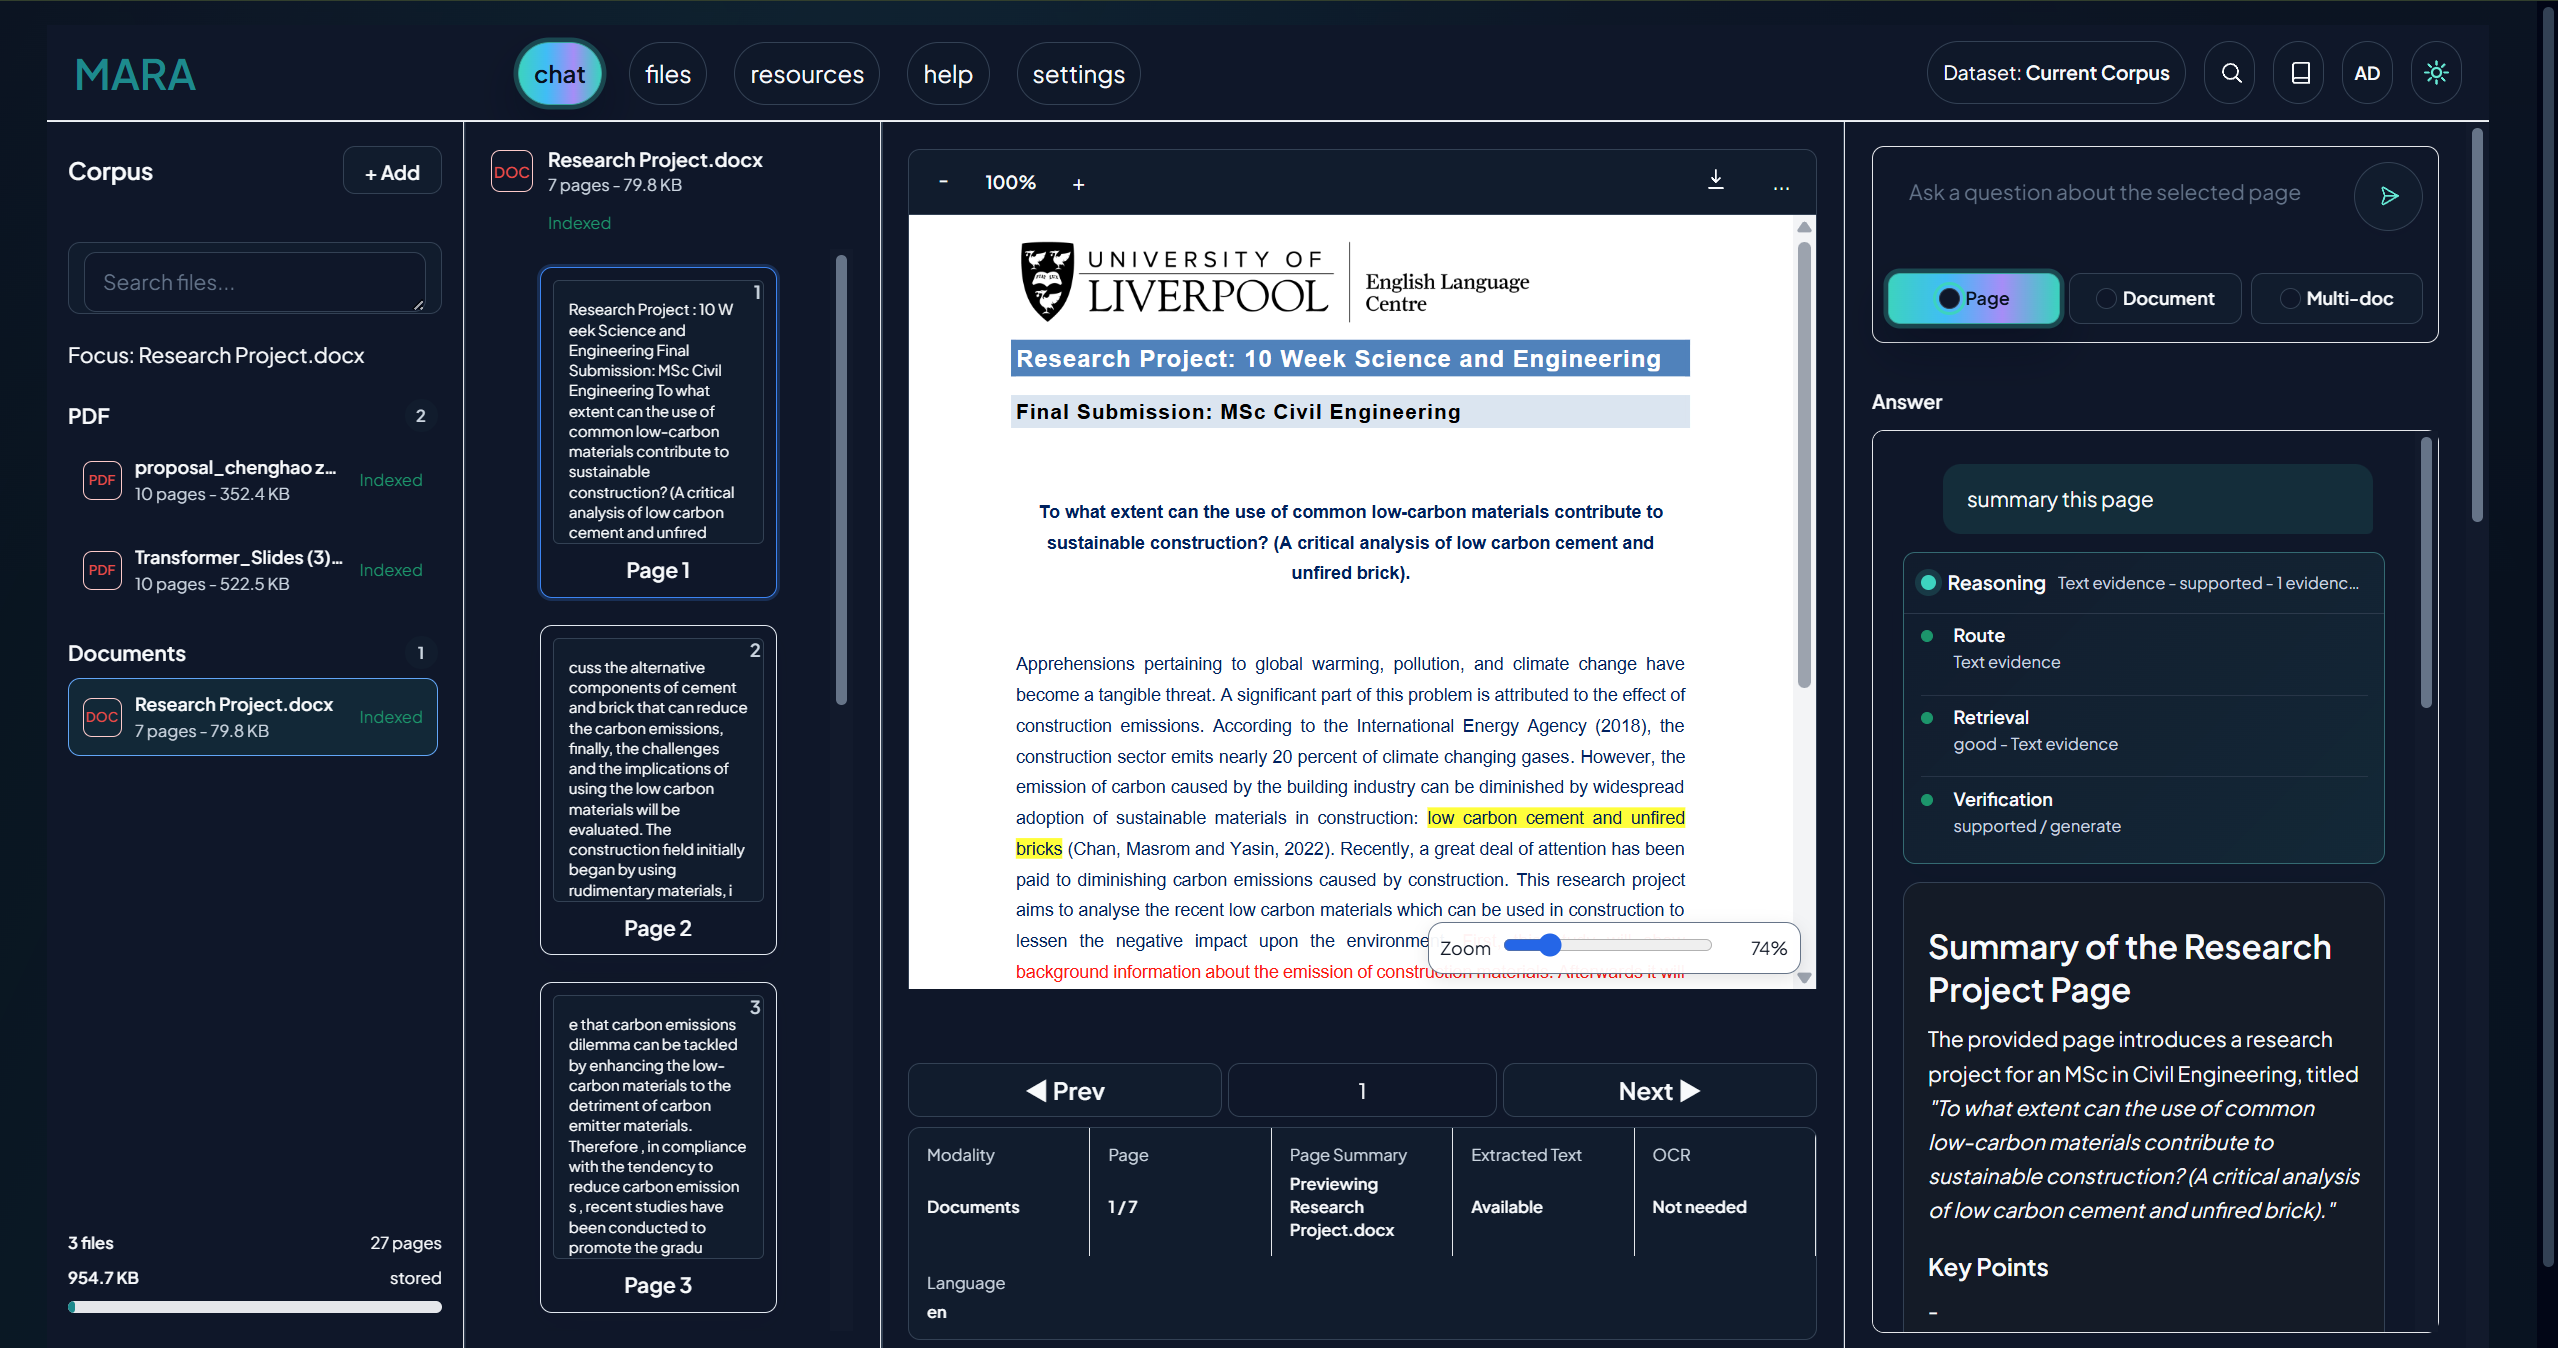
\includegraphics[width=0.85\textwidth]{figures/mara-ui-qa.png}
\caption{Primary MARA demo interface on the non-sensitive document
\texttt{ResearchProject.docx}. The interface combines source
selection, page preview, routed answering, and a compact reasoning
status panel that reports the selected route, retrieval status, and
verification outcome.}
\label{fig:ui}
\end{figure*}

\section{Introduction}
\Xiao{Large language models (LLMs) are increasingly popular as a tool for information seeking \citep{brown2020language, openai2024gpt4technicalreport}.}
Document question answering is increasingly built on
retrieval-augmented generation (RAG), which grounds
language-model outputs in external evidence
\citep{lewis2020rag, karpukhin2020dpr, gao2023rag}.
\Xiao{Despite growing interest in reliability-oriented RAG, route-aware evidence selection, citation grounding, and abstention for multimodal document collections remain understudied.}

\Xiao{Recent developments, such as ALCE, Self-RAG, Adaptive-RAG, CRAG, RAGTruth \citep{DBLP:conf/emnlp/GaoYYC23, asai2023selfrag,jeong2024adaptiverag, yan2024crag, niu2024ragtruth} have improved the reliability of retrieval-augmented generation. However, }
practical document collections are not purely
textual: answers may depend on tables, figures, slide
images, page layout, or evidence distributed across
multiple pages and documents
\citep{tanaka2023slidevqa, faysse2024colpali,
dong2025mmdocrag}.
Fixed retrieve-then-generate pipelines can therefore
select an unsuitable evidence path, while weak retrieval
can produce unsupported answers. Unlike
previous works, our approach aims
to bridge that gap by constructing %, motivatingcitation-aware generation, adaptive retrieval, evidenceverification, and abstention\citep{GaoYYC23, asai2023selfrag,jeong2024adaptiverag, yan2024crag, niu2024ragtruth}.A practical document QA system should therefore choosean appropriate route, expose the evidence and citations it used, and abstain when support is insufficient. MARA, short for Multimodal Agentic Retrieval and Answering, is 
a local-first multimodal document QA workbench built for this setting. %It is not a new foundation model. Instead, 
It is a demonstrable system that extends a Kotaemon-style local QA baseline \citep{kotaemon}. The inherited baseline already supports file upload, model configuration, and a standard document QA flow. MARA focuses on the controller-centred extension: route-aware retrieval and answering, evidence checking, citation, and trace observability, multimodal routes, shared Web/CLI workflows, and benchmark-backed evaluation of these behaviours.MARA targets researchers, students, and technical
professionals who require local and inspectable QA over
mixed document collections.

%The distinguishing idea is a Self-RAG-inspired controller. 
\Xiao{We address critical questions about the retrieval routing and observability of document QA inspired by Self-RAG \citep{asai2023selfrag}. We introduce MARA, a local-first multimodal document QA workbench for observable, traceable routing decisions across text, visual, hybrid, and graph-based retrieval evidence paths. MARA is built on Qwen/Qwen3-8B as the text generation backend and BAAI/bge-m3 as the text retrieval backend, and is evaluated on a benchmark spanning 41 completed artefact sets and 3,540 prediction records across QASPER, ALCE-ASQA, and MMDocRAG.}

Our result show that MARA perform competitive on text-heavy and citation-grounded tasks across standard metrics such as false-abstention rate and F1. MARA records 0.00\% false abstenti on ALCE-ASQA, while improving F1 and citation recall on fixed text retrieval and document-QA generation. To demonstrate real-world applicability, we develop a research demo showcasing in Figure~\ref{fig:ui}. 

%: source selection,
%page inspection, routed answering, and compact route, retrieval,
%and verification status. Full citation, evidence-bundle, andcontroller-trace records remain in runtime and benchmark artefacts.

%Self-RAG treats retrieval and critique as explicit decisions \citep{asai2023selfrag}; MARA adapts this idea at the system level. Rather than training a model with reflection tokens, MARA records ordinary program decisions: whether to retrieve, which route to use, whether evidence is adequate, whether a higher-cost route is justified, whether to switch routes, and whether to abstain. This design keeps the system feasible as a local prototype while preserving the core research question: can route-aware control make a document QA workbench more transparent and reliable than a fixed RAG pipeline?

This paper makes three contributions:
\begin{itemize}
    \item A local-first multimodal document QA workbench exposing the same QA workflow through Web UI, local CLI, and optional agent-platform wrappers.
    \item A traceable Self-RAG-inspired controller that selects among text, visual, hybrid, CRAG-guarded, graph, direct, and abstention behaviours using route probes, heuristic route-scoring proxies, workflow-cost annotations, evidence checks, route switching, and verification traces.
    \item A benchmark-backed demonstration using a full-system benchmark to compare routes across QASPER, ALCE-ASQA, and MMDocRAG, with additional routes and datasets analysed diagnostically.
\end{itemize}

\section{Approach}

\subsection{Local-First Document QA Workbench}

MARA has three user surfaces built around one DocQA runtime. The Web UI provides the primary demo: users add documents,
select sources, inspect pages, ask questions, examine answers,
and view compact route, retrieval, and verification status. The CLI supports non-UI workflows such as indexing, file inspection, one-shot QA, chat, sessions, sources, notes, and artefacts. Optional platform skills wrap those documented commands for Codex and Claude Code environments. These surfaces are designed to reuse the same DocQA runtime and persisted state, reducing Web/CLI drift, although the implementation still contains multiple entrypoints that require contract tests.

The implementation boundary is deliberately conservative. MARA is a branded fork of Kotaemon: internal package names such as \texttt{kotaemon}, \texttt{ktem}, and \texttt{slide\_cli} remain for compatibility, while the public product commands are \texttt{MARA} and \texttt{MARA-cli}. Kotaemon provides the basic local QA substrate: document upload, model and embedding configuration, indexing, and a conventional document QA path. MARA keeps this substrate, but adds a controller layer and a benchmark layer around it. The controller layer builds route decisions, workflow plans, evidence bundles, retrieval adequacy decisions, verification decisions, guardrail payloads, and controller traces. The benchmark layer converts public or local datasets into route manifests and evaluates the same runtime used by the UI and CLI. This separation is important for the paper claim: MARA does not claim novelty for ordinary file upload or model configuration, but for the route-aware extension and its observability.

\begin{figure}[!t]
\centering
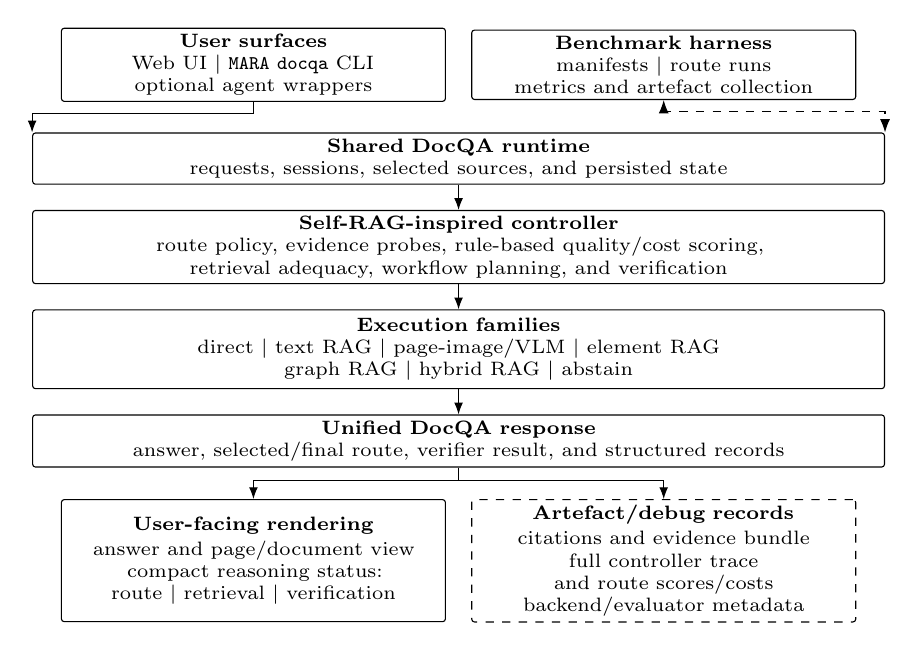
\begin{tikzpicture}[
    font=\scriptsize,
    node distance=3.2mm and 3.2mm,
    box/.style={
        draw,
        rounded corners=1pt,
        align=center,
        inner sep=2.1pt,
        minimum height=6.5mm
    },
    topbox/.style={
        box,
        text width=0.39\columnwidth
    },
    widebox/.style={
        box,
        text width=0.88\columnwidth
    },
    routebox/.style={
        box,
        text width=0.88\columnwidth,
        minimum height=10mm
    },
    outbox/.style={
        box,
        text width=0.39\columnwidth,
        minimum height=15.5mm
    },
    artefactbox/.style={
        outbox,
        dashed
    },
    flow/.style={
        -{Latex[length=1.5mm]},
        thin
    },
    benchmarkflow/.style={
        <->,
        >=Latex,
        thin,
        dashed
    }
]

% Entry points
\node[topbox] (surfaces) {
    \textbf{User surfaces}\\
    Web UI $\mid$ \texttt{MARA docqa} CLI\\
    optional agent wrappers
};

\node[topbox, right=3.2mm of surfaces] (benchmark) {
    \textbf{Benchmark harness}\\
    manifests $\mid$ route runs\\
    metrics and artefact collection
};

% Centre the runtime beneath the two entry boxes.
\path (surfaces.south east) -- (benchmark.south west)
    node[midway, below=4mm, widebox] (runtime) {
        \textbf{Shared DocQA runtime}\\
        requests, sessions, selected sources, and persisted state
    };

\node[widebox, below=of runtime] (controller) {
    \textbf{Self-RAG-inspired controller}\\
    route policy, evidence probes, rule-based quality/cost scoring,\\
    retrieval adequacy, workflow planning, and verification
};

\node[routebox, below=of controller] (routes) {
    \textbf{Execution families}\\
    direct $\mid$ text RAG $\mid$ page-image/VLM $\mid$ element RAG\\
    graph RAG $\mid$ hybrid RAG $\mid$ abstain
};

\node[widebox, below=of routes] (response) {
    \textbf{Unified DocQA response}\\
    answer, selected/final route, verifier result,
    and structured records
};

% Different levels of observability
\node[
    outbox,
    below left=4mm and 1.6mm of response.south
] (uiout) {
    \textbf{User-facing rendering}\\[1pt]
    answer and page/document view\\
    compact reasoning status:\\
    route $\mid$ retrieval $\mid$ verification
};

\node[
    artefactbox,
    below right=4mm and 1.6mm of response.south
] (Artefacts) {
    \textbf{Artefact/debug records}\\[1pt]
    citations and evidence bundle\\
    full controller trace and route scores/costs\\
    backend/evaluator metadata
};

% Data and control flow
\draw[flow]
    (surfaces.south)
    -- ++(0,-1.5mm)
    -| (runtime.north west);

\draw[benchmarkflow]
    (benchmark.south)
    -- ++(0,-1.5mm)
    -| (runtime.north east);

\draw[flow] (runtime) -- (controller);
\draw[flow] (controller) -- (routes);
\draw[flow] (routes) -- (response);

\draw[flow]
    (response.south)
    -- ++(0,-1.6mm)
    -| (uiout.north);

\draw[flow]
    (response.south)
    -- ++(0,-1.6mm)
    -| (Artefacts.north);

\end{tikzpicture}

\caption{MARA architecture. The Web UI, CLI, and benchmark
harness share one DocQA runtime. The UI renders compact
route, retrieval, and verification status, while full evidence
and trace records remain in runtime artefacts.}
\label{fig:architecture}
\end{figure}


The Web UI is built as a workbench rather than a chat-only interface, following the practical advantages of Gradio-style local applications \citep{gradio}. The primary demo screen exposes source management, a page
viewer, and a route-aware QA panel. The answer panel displays
a compact reasoning summary consisting of the selected
route or evidence category, retrieval status, and verification
outcome. Full evidence bundles, citation records, route scores,
and controller-trace fields remain available to benchmark and
debugging workflows rather than being rendered in full in the
main UI. Local-first execution also supports a clearer security story: the system can run with local files and local or explicitly configured model endpoints, reducing hidden data movement and making backend metadata visible, which is aligned with LLM application risk guidance \citep{owaspLLM}.

\subsection{Self-RAG-Inspired Routing Controller}

\paragraph{Route vocabularies and mapping.}
MARA distinguishes internal execution families from benchmark configurations. Internal identifiers such as \texttt{doc\_text}, \texttt{doc\_page\_image}, and \texttt{hybrid} determine the executor and evidence type, whereas benchmark IDs may also specify a backend, graph mode, agent mode, or verification policy. Fixed configurations map to one family, backend variants may share a family, and \texttt{controller\_auto} or \texttt{crag\_guarded} can select among several families. Result tables report the requested benchmark configuration, while the controller trace records the selected and final execution routes. Table~\ref{tab:route-mapping} gives the complete mapping.


\begin{table*}[t]
\centering
\begingroup
\footnotesize
\setlength{\tabcolsep}{4pt}
\renewcommand{\arraystretch}{1.12}
\begin{tabularx}{\textwidth}{@{}
>{\raggedright\arraybackslash}p{0.20\textwidth}
>{\raggedright\arraybackslash}p{0.25\textwidth}
>{\raggedright\arraybackslash}p{0.16\textwidth}
>{\raggedright\arraybackslash}X@{}}
\toprule
\rowcolor{gray!15}
\begin{tabular}[t]{@{}l@{}}Benchmark route\\ID\end{tabular}
& \begin{tabular}[t]{@{}l@{}}Internal family\\(\texttt{legacy\_route})\end{tabular}
& \begin{tabular}[t]{@{}l@{}}Canonical trace\\\texttt{route}\end{tabular}
& Configuration meaning \\
\midrule
\texttt{direct\_answer}
& \texttt{direct}
& \texttt{direct\_answer}
& Fixed no-retrieval baseline. \\

\texttt{text\_rag}
& \texttt{doc\_text}
& \texttt{text\_rag}
& Fixed text retrieval and document-QA generation. \\

\texttt{page\_image\_rag\_smoke}
& \texttt{doc\_page\_image}
& \texttt{page\_image\_rag}
& Deterministic page-image smoke/evidence-only configuration. \\

\texttt{page\_image\_rag\_vlm}
& \texttt{doc\_page\_image}
& \texttt{page\_image\_rag}
& The same execution family with a configured visual retriever and VLM generator. \\

\texttt{element\_rag}
& \texttt{doc\_element}
& \texttt{element\_rag}
& Fixed document-element evidence path. \\

\texttt{graph\_rag\_local}
& \texttt{graph\_global}
& \texttt{graph\_rag}
& Local graph-mode experimental configuration. \\

\texttt{graph\_rag\_global}
& \texttt{graph\_global}
& \texttt{graph\_rag}
& Global-summary graph-mode experimental configuration. \\

\texttt{hybrid\_rag}
& \texttt{hybrid}
& \texttt{hybrid\_rag}
& Fixed fusion of text, page-image, and element evidence. \\

\texttt{controller\_auto}
& Dynamic choice among \texttt{doc\_text}, \texttt{hybrid}, \texttt{doc\_page\_image}, \texttt{doc\_element}, and \texttt{graph\_global}.
& Canonical route of the selected family
& Automatic routing with light verification; the executed family can differ across examples. \\

\texttt{crag\_guarded}
& The same dynamic candidate set; the final route may be \texttt{abstain}.
& Canonical route of the selected/final family
& Automatic routing with stricter verification and guarded recovery or abstention. \\
\bottomrule
\end{tabularx}
\endgroup
\caption{Mapping between benchmark-facing route IDs and MARA's internal execution families. A benchmark ID denotes an experimental configuration, whereas the controller trace records the execution family actually selected and finally used. Retrieval-only diagnostics are outside this table because they do not execute a complete QA generation route.}
\label{tab:route-mapping}
\end{table*}

The five configurations highlighted in the main results are \texttt{controller\_auto}, \texttt{text\_rag}, \texttt{crag\_guarded}, \texttt{hybrid\_rag}, and \texttt{page\_image\_rag\_vlm}. The controller is rule-based rather than trained. It begins with a fixed, planner-supplied, or heuristic route; when route probes are available, a rule-based scorer compares allowed routes using uncalibrated quality and cost proxies. These values support inspectable selection and cost gating, not prediction of true answer accuracy, latency, or monetary cost.

Routing follows the question and available evidence. Text is the default for ordinary QA; visual cues can activate page-image routes; structured calculations and tables can justify hybrid evidence; and global summary or comparison tasks can use graph context. Visual and hybrid routes remain higher-cost options whose usefulness depends on backend health and probe evidence.

The trace records the requested, selected, and final routes, routing rationale, evidence adequacy, verification outcome, optional score and cost fields, and any recovery or abstention decision. If retrieval or verification fails, MARA can switch routes and retry once; if evidence remains insufficient, it abstains. Full trace fields are retained for benchmarking and debugging rather than rendered in the main UI.

\begin{center}
\refstepcounter{algorithm}\label{alg:controller}
\fbox{\begin{minipage}{0.94\linewidth}
\scriptsize
\textbf{Algorithm \thealgorithm: MARA route selection}\\[1mm]
\begin{tabularx}{\linewidth}{@{}r@{\quad}X@{}}
1 & \textbf{Input:} question $q$, selected sources $S$, route policy $p$ \\
2 & \textbf{Output:} answer, citations, evidence bundle, route trace \\
3 & features $\leftarrow$ inspect task type, scope, modalities, backend health \\
4 & planner\_route $\leftarrow$ fixed, structured-planner, or heuristic route \\
5 & \textbf{if} route probing is enabled \textbf{then} \\
6 & \hspace*{1em} probes $\leftarrow$ probe text, visual, element, graph evidence \\
7 & \hspace*{1em} scores $\leftarrow$ rule-based cost-aware scorer(probes, features, allowed routes, dataset family, latency budget) \\
8 & \hspace*{1em} route $\leftarrow$ highest-scoring allowed non-skipped route \\
9 & \textbf{else} \\
10 & \hspace*{1em} route $\leftarrow$ planner\_route \\
11 & \textbf{end if} \\
12 & plan $\leftarrow$ build workflow steps with cost units \\
13 & evidence $\leftarrow$ retrieve and normalise route evidence \\
14 & verify $\leftarrow$ check retrieval adequacy and answer support \\
15 & \textbf{if} verify fails and recovery route is available \textbf{then} \\
16 & \hspace*{1em} switch route and retry retrieval once \\
17 & \textbf{else if} verify fails \textbf{then} \\
18 & \hspace*{1em} abstain with evidence status and reason \\
19 & \textbf{end if} \\
20 & \textbf{return} answer, citations, evidence, route decision, verifier state \\
\end{tabularx}
\vspace{0.5mm}

\emph{The quality and cost fields are uncalibrated controller proxies, not learned or calibrated estimates of true answer correctness, latency, or monetary cost.}
\end{minipage}}
\end{center}

The design is Self-RAG-inspired at the system level: retrieval, route choice, critique, recovery, and abstention are explicit program decisions. The stricter \texttt{crag\_guarded} configuration applies tighter verification, making its false-abstention trade-off directly measurable.

\subsection{Benchmark Harness and Trace Artefacts}

MARA treats benchmarking as part of the system approach rather than as a detached leaderboard script. The harness converts public or local datasets into route manifests, runs the same DocQA runtime used by the UI and CLI, and stores per-example predictions, retrieval traces, documents, route metrics, and summaries. Each run specifies a dataset, shard, route request, allowed routes, backend metadata, verification mode, citation mode, and benchmark role. %Metrics include exact match, token F1, local dataset-native score, citation recall, page hit, unsupported-claim rate, false-abstention rate, route-switch rate, errors, timeout counts, and latency.

The benchmark separates local dataset-native and MARA diagnostic scores from paper-grade external evaluator scores, because no official external evaluator was configured for the main synthesis. Reproducibility metadata includes the synthesis script, input job manifest, generated table files, skipped and complete artefact status, route metrics, backend health fields, and evaluator authority status. This design keeps the demo paper claim inspectable: route-aware behaviour is visible in the UI, reproducible through command-line artefacts, and measurable across dataset families.

\section{Experiments and Results}

\subsection{Experiment Setup}
The configured backends also matter for interpretation. The text routes used Qwen/Qwen3-8B \citep{yang2025qwen3} as the main text generator and BAAI/bge-m3 \citep{chen2024bgem3} as the text retriever in the recorded metadata. The default local visual retriever is a deterministic late-interaction-style smoke backend over OCR, captions, text, and visual tokens; ColPali/ColQwen-style HTTP retrievers are configurable backends rather than a default guarantee. Page-image generation uses local Qwen3-VL \citep{bai2025qwen3vl} only when the OpenAI-compatible VLM endpoint is configured and healthy; otherwise the route can fall back to evidence-only visual output. These details are not fixed product requirements, but backend conditions that must be read from each benchmark run's metadata.


%The main quantitative evidence comes from the full-system benchmark. The synthesis loaded 41 complete artefact sets and 3,540 per-example prediction records. Required synthesis tables for main results, route decisions, failures/latency/backend metadata, paired route deltas, bootstrap confidence intervals, controller oracle regret, and win/loss/tie comparisons were generated successfully.

\subsubsection{Baselines}
\Xiao{We compare \texttt{controller\_auto} against the fixed \texttt{text\_rag} route as the primary baseline, along with \texttt{crag\_guarded}, \texttt{hybrid\_rag}, and \texttt{page\_image\_rag\_vlm} as route-specific comparisons. \texttt{direct\_answer} (no retrieval) serves as a no-evidence control condition.}
%The paper prioritises three datasets for the demo narrative. QASPER represents text-heavy scientific document QA \citep{dasigi2021qasper}. ALCE-ASQA represents citation-grounded answer generation \citep{GaoYYC23}. MMDocRAG represents multimodal document QA with text, page-image, hybrid, and element routes \citep{dong2025mmdocrag}. FinanceBench, RAGTruth, and SlideVQA are reported in the appendix as diagnostic full-system datasets, while ViDoRe remains a separate retrieval diagnostic rather than part of the 41-set generation benchmark.
\subsubsection{Evaluation Metrics}
\Xiao{We employ a diverse set of metrics to evaluate models’ performance across the full-system benchmark. Metrics include exact match, token F1, local dataset-native score, citation recall, page hit, unsupported-claim rate, false-abstention rate, route-switch rate, errors, timeout counts, and latency.}

%The configured backends also matter for interpretation. The text routes used Qwen/Qwen3-8B \citep{yang2025qwen3} as the main text generator and BAAI/bge-m3 \citep{chen2024bgem3} as the text retriever in the recorded metadata. The default local visual retriever is a deterministic late-interaction-style smoke backend over OCR, captions, text, and visual tokens; ColPali/ColQwen-style HTTP retrievers are configurable backends rather than a default guarantee. Page-image generation uses local Qwen3-VL \citep{bai2025qwen3vl} only when the OpenAI-compatible VLM endpoint is configured and healthy; otherwise the route can fall back to evidence-only visual output. These details are not fixed product requirements, but backend conditions that must be read from each benchmark run's metadata.

\subsection{Results}

Table~\ref{tab:main-results} reports selected route-level results on a 0--100 scale; %the underlying artefact files store scores in 0--1 form. 
False abstention is also shown as a percentage. Citation denotes metadata citation recall, and Native denotes the local dataset-native score used by the benchmark harness; inline and metadata citation recall are equal or nearly equal for QASPER and ALCE-ASQA in the synthesis.

\begin{table*}[t]
\centering
\small
\begin{tabular}{llrrrrrr}
\toprule
\rowcolor{gray!15}
Dataset & Route & N & F1 & Native & Citation & Page hit & False abs. \\
\midrule
QASPER & controller\_auto & 200 & 21.43 & 21.43 & 89.65 & -- & 0.00 \\
QASPER & text\_rag & 200 & 21.44 & 21.44 & 90.91 & -- & 1.50 \\
QASPER & crag\_guarded & 200 & 20.06 & 20.06 & 89.65 & -- & 6.00 \\
\midrule
ALCE-ASQA & controller\_auto & 200 & 25.74 & 77.07 & 95.50 & -- & 0.00 \\
ALCE-ASQA & text\_rag & 200 & 26.68 & 77.14 & 95.50 & -- & 0.00 \\
ALCE-ASQA & crag\_guarded & 200 & 15.16 & 63.20 & 95.50 & -- & 46.00 \\
\midrule
MMDocRAG & controller\_auto & 120 & 34.60 & 34.60 & 67.99 & 82.50 & 0.00 \\
MMDocRAG & text\_rag & 120 & 35.44 & 35.44 & 68.62 & 81.67 & 5.83 \\
MMDocRAG & hybrid\_rag & 120 & 33.99 & 33.99 & 30.77 & 58.33 & 0.00 \\
MMDocRAG & page\_image\_rag\_vlm & 120 & 16.38 & 16.38 & 48.41 & 56.67 & 0.00 \\
\bottomrule
\end{tabular}
\caption{Selected route-level results from the full-system benchmark.}
\label{tab:main-results}
\end{table*}

Table~\ref{tab:main-results} supports three observations. First, the controller stays competitive with text RAG on QASPER and ALCE-ASQA, where the evidence is largely textual. The text baseline remains slightly stronger by F1 on ALCE-ASQA, so the honest claim is not that the controller dominates text RAG, but that the route-aware system maintains comparable answer quality while exposing trace and guardrail metadata. Second, CRAG-guarded mode demonstrates the cost of strict evidence checks: it reduces unsupported-claim risk in some settings but can increase false abstention, especially on ALCE-ASQA. Third, MMDocRAG shows the value of measuring multimodal route behaviour directly. Text RAG and controller-auto are the strongest quality routes. %while hybrid and page-image/VLM routes expose visual and multimodal evidence paths that remain useful for diagnosis and future optimisation.

Paired comparisons reinforce this cautious interpretation. On QASPER, controller-auto was essentially tied with text RAG by F1 and improved over CRAG-guarded by a mean paired delta of 1.38 points on the 0--100 scale. On ALCE-ASQA, controller-auto trailed text RAG by 0.94 points but improved over CRAG-guarded by 10.57 points. On MMDocRAG, controller-auto trailed text RAG by 0.84 points but exceeded page-image/VLM by 18.22 points and element RAG by 29.03 points. The win/loss/tie tables show that many examples are ties, which is expected for short-answer and citation-heavy tasks. The main paper therefore treats the benchmark as a diagnostic system evaluation rather than a claim of state-of-the-art accuracy.

\section{Use Case}

The UI walkthrough presents a complete QA loop. A user
opens the local application, indexes the non-sensitive
demonstration document \texttt{ResearchProject.docx},
selects the source and QA scope, asks a question, and
receives a routed answer. The central viewer displays the
selected source page. In the right-hand panel, a compact
reasoning-status card reports the route or evidence category,
retrieval status, and verification outcome. Richer evidence,
citation, and controller-trace records are available through
the runtime and benchmark artefacts. Figure~\ref{fig:ui}
shows this workflow.

% \begin{figure*}[t]
% \centering
% 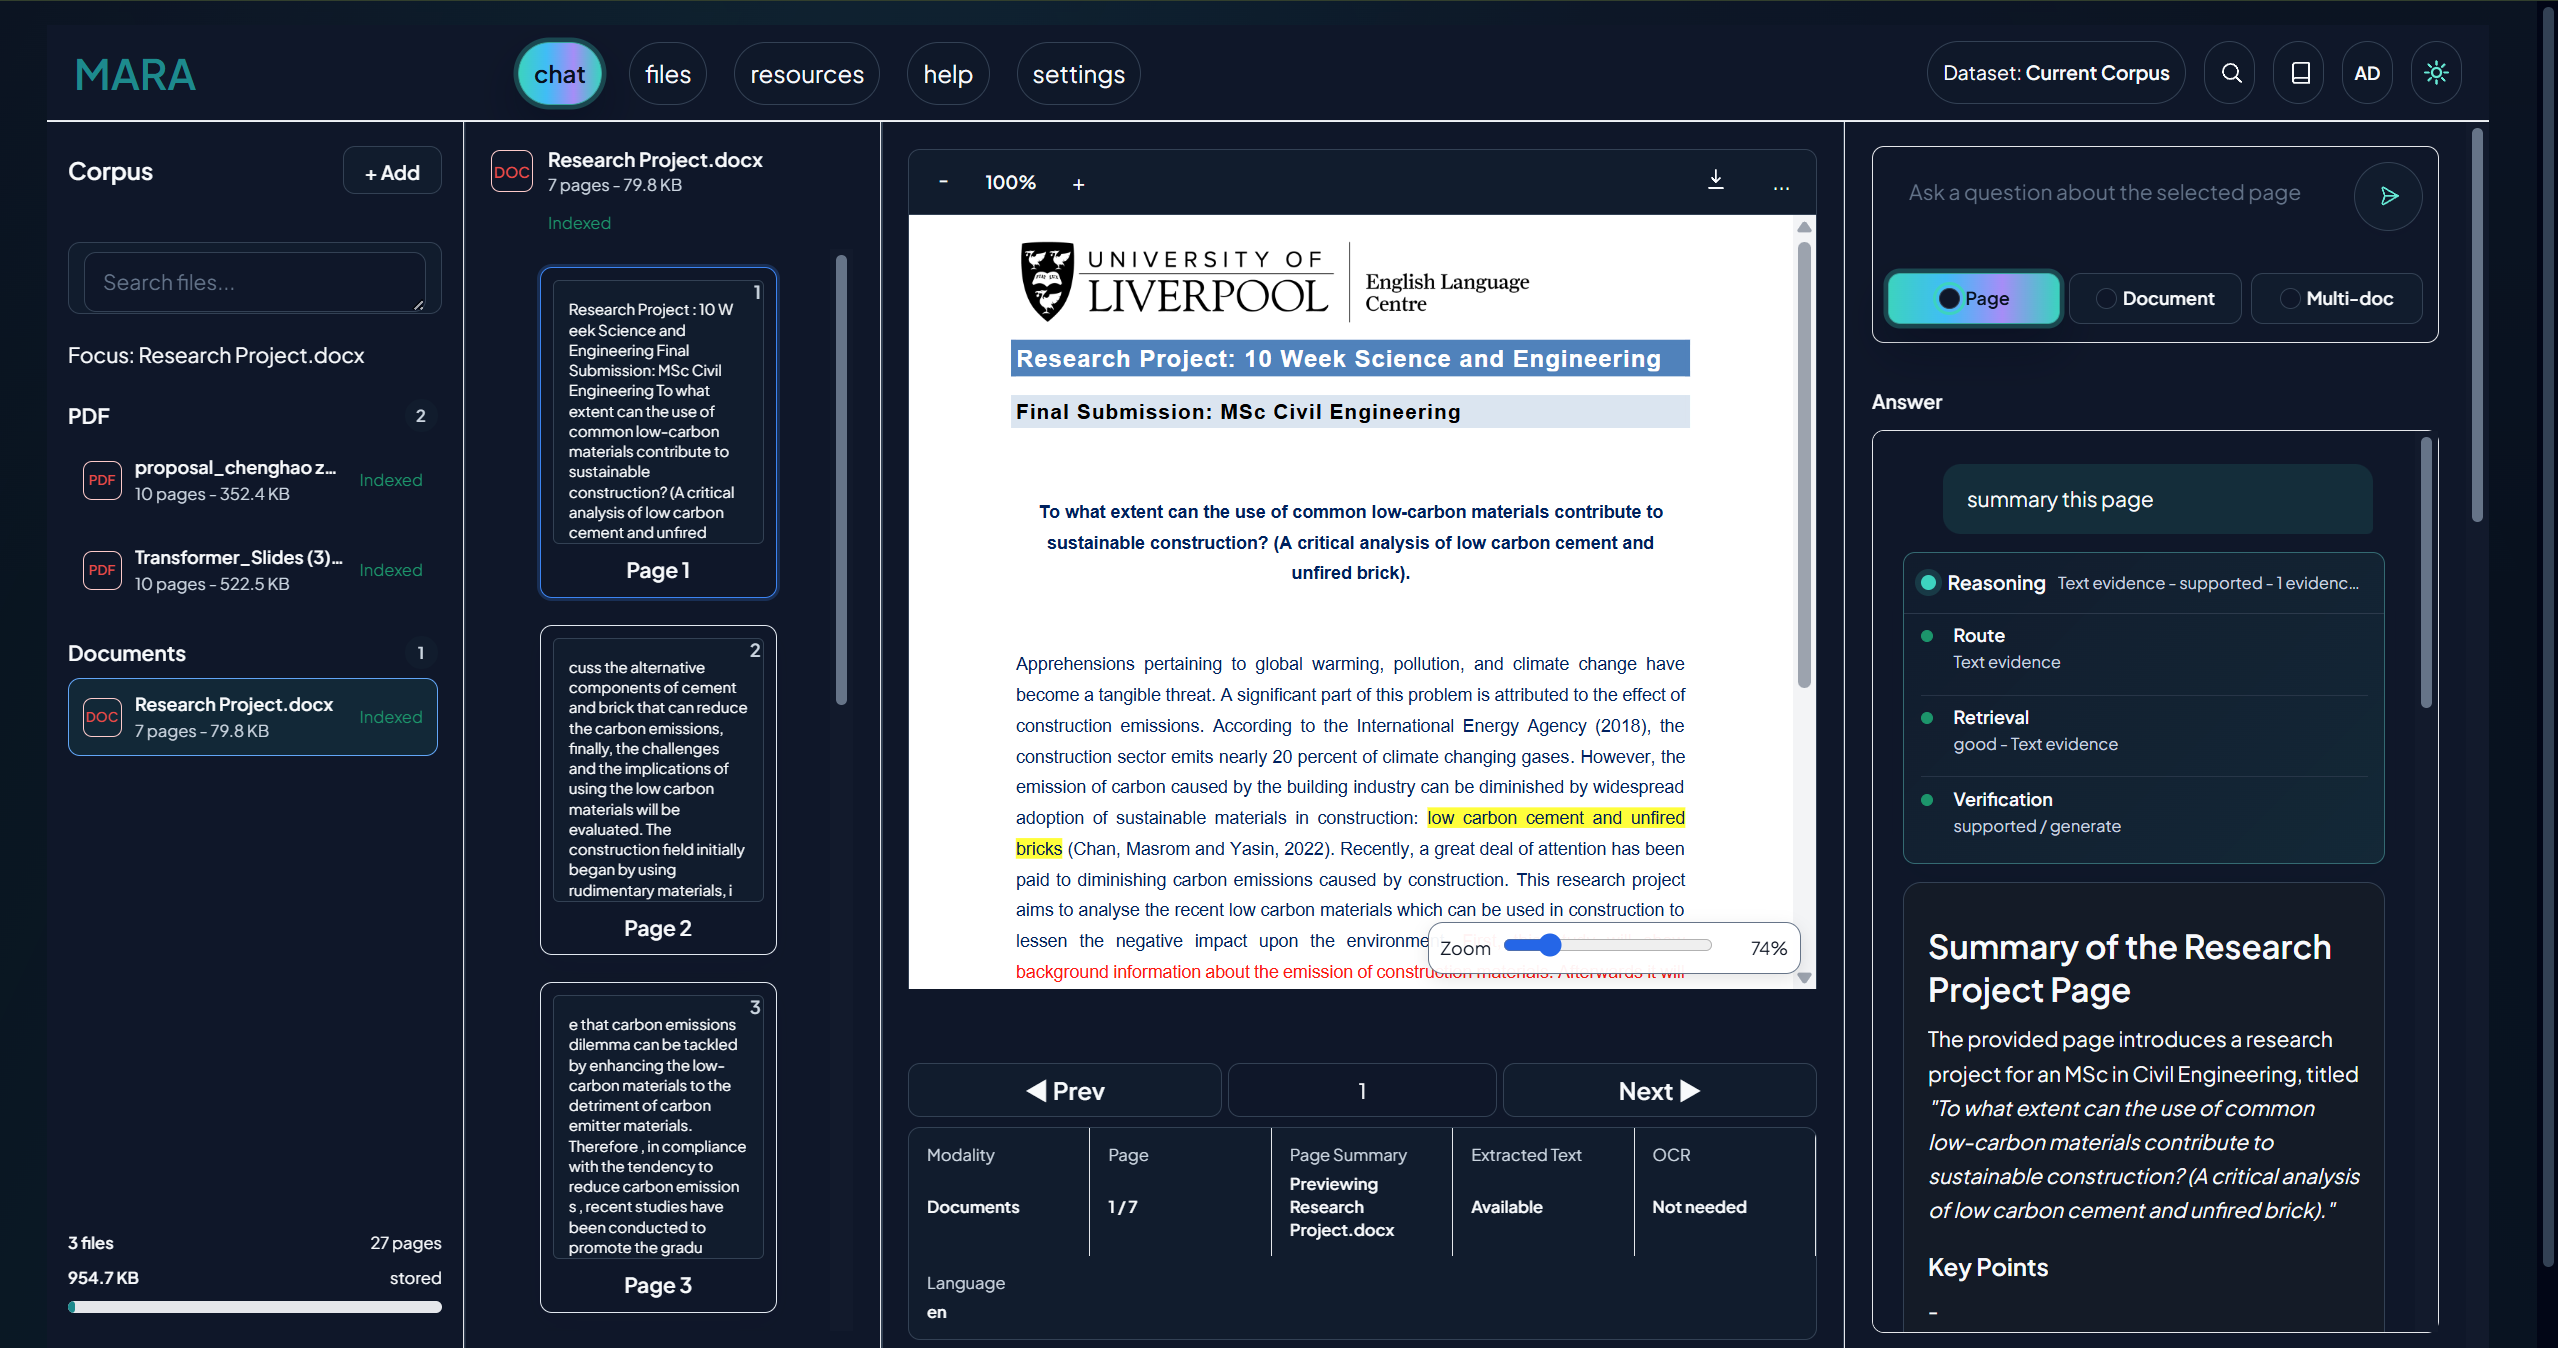
\includegraphics[width=\textwidth]{figures/mara-ui-qa.png}
% \caption{Live MARA UI screenshot on the non-sensitive demonstration document \texttt{ResearchProject.docx}: source selection, page preview, routed answer, evidence metadata, retrieval status, and controller trace in one QA workflow.}
% \label{fig:ui}
% \end{figure*}

The CLI walkthrough supports the same scenario without a browser:
\begin{quote}\small
\texttt{MARA docqa index ./docs/report.pdf}\\
\texttt{MARA docqa files}\\
\texttt{MARA docqa ask -{}-file report.pdf -{}-reasoning mara -{}-prompt "..."}
\end{quote}
The benchmark walkthrough starts from route manifests and produces prediction records, route metrics, and synthesis tables, demonstrating that route-aware behaviour is not only visible in the UI, but also reproducible through a public release tag and supplementary benchmark bundle whose synthesis script, backend metadata, and evaluator status are recorded in the appendix.

\Xiao{These three surfaces demonstrate the same route-aware behaviour from complementary angles. The UI scenario exposes document selection, page inspection,
answer generation, and the compact route, retrieval, and
verification summary. The CLI scenario confirms that \texttt{MARA docqa} is a reproducible surface over the same runtime rather than a separate implementation, and the benchmark scenario connects this UI-visible trace to aggregate route metrics. }
%The intended demonstration has three short scenarios. First, a UI scenario indexes \texttt{ResearchProject.docx} and asks a question whose answer requires source-grounded evidence. The demo highlights document selection, answer generation, citations, and the route trace. Second, a CLI scenario repeats a similar workflow without launching the browser, showing that \texttt{MARA docqa} is not a separate implementation but a reproducible surface over the same runtime. Third, a benchmark scenario opens the full-system synthesis tables and connects the UI-visible route trace to aggregate route metrics. 
The Codex and Claude Code wrappers are shown only as optional platform integrations, with details left to the appendix.

\paragraph{System availability and license.}

\ifmaraanonymous
The anonymized package includes an installable MARA archive, benchmark
artefacts, and a short demonstration video. MARA is distributed under
the Apache License 2.0; third-party resources retain their original
licenses. Public links are omitted during anonymous review.
\else
The MARA source code, installation instructions, and
downloadable artefacts are available from the project
repository\footnote{\url{https://github.com/262412/MARA}}.
The version evaluated in this paper is archived as the
\texttt{v0.0.40} release
\footnote{\url{https://github.com/262412/MARA/releases/tag/v0.0.40}}.
A short demonstration video is available online
\footnote{\url{https://youtu.be/owRaHCzSVNg}}. It demonstrates the primary Web UI workflow, including
source selection, page preview, page- and document-level
question answering, and compact route, retrieval, and
verification status. The CLI and benchmark workflows are
documented in the paper and public release. MARA is released under the Apache License 2.0 and
retains the upstream Kotaemon attribution in
\texttt{LICENSE.txt} and \texttt{NOTICE}. Third-party
models, datasets, and documents remain subject to their
respective licenses.

\section{Related Work}

\subsection{Route-Aware RAG and Verification}

RAG systems retrieve external evidence before generation and are a standard pattern for knowledge-intensive QA \citep{lewis2020rag,karpukhin2020dpr,gao2023rag}. Their weakness is that retrieval is often treated as a fixed step. MARA instead treats route choice, evidence adequacy, and abstention as observable controller decisions.

Self-RAG motivates this design by learning when to retrieve and when to critique retrieved evidence \citep{asai2023selfrag}. MARA does not reproduce Self-RAG training. It uses the decision structure as a system-level controller. Adaptive RAG systems similarly motivate route selection by question type and difficulty \citep{jeong2024adaptiverag}. Corrective RAG (CRAG) highlights the need to judge retrieval quality before generation \citep{yan2024crag}; MARA includes guarded retrieval and verification states that can retry, switch, or abstain.

\subsection{Multimodal Document QA and Workbenches}

Multimodal document QA adds further route pressure. Page-image retrieval methods such as ColPali preserve layout and visual details that OCR chunks can lose \citep{faysse2024colpali}. MMDocRAG benchmarks retrieval-augmented multimodal generation for document QA and exposes text/visual trade-offs \citep{dong2025mmdocrag}. GraphRAG methods are useful for global summarisation and cross-document questions \citep{edge2024graphrag}, while datasets such as QASPER, ALCE, RAGTruth, and SlideVQA expose long-document evidence, citations, hallucination risk, and visual QA \citep{dasigi2021qasper,DBLP:conf/emnlp/GaoYYC23,niu2024ragtruth,tanaka2023slidevqa}.

MARA sits between these lines of work. It is a local workbench with practical UI and CLI affordances, but its main research-facing object is the controller trace: route, evidence, verification, cost, and abstention decisions that can be inspected by a user and measured by a benchmark harness.

\section{Conclusion}
\Xiao{In this work, we introduce MARA, a local-first multimodal document QA workbench. It integrates a Self-RAG-inspired routing controller, shared UI/CLI surfaces, and a benchmark harness into a single, inspectable system. Our full-system benchmark draws on six datasets, spanning 41 completed artefact sets and 3,540 prediction records. MARA remains competitive on text-heavy and citation-grounded tasks, suggesting that route-aware control preserves competitive answer quality while adding observability. To showcase real-world applicability, we develop a demonstration system featuring MARA’s route-aware document QA capabilities, paving the way for broader adoption of local-first, observable document QA workbenches that reduce hidden data movement while making retrieval and answering behaviour transparent to users.}
%MARA's strongest current result is not a single benchmark number. It is the integration of UI, CLI, controller trace, evidence records, and route-level evaluation into one local-first system. The controller makes routing inspectable: users can see not only an answer, but also the route, evidence, citations, verifier status, workflow cost, optional planner scoring fields, recovery routes, and abstention behaviour.

%The limitations are important. The controller is rule-based by default: it combines heuristic planning with route-probe scoring when probes are available, but it is not a trained or calibrated router. Element and graph routes are implemented as prototype or scoped routes and need stronger evidence indexes and task-specific evaluation before they should be framed as mature. Page-image/VLM support depends on configured visual retrieval and generation backends, which can be slower than text routes and may run in evidence-only mode when the VLM backend is unavailable. The full-system benchmark did not use paper-grade external evaluators; it reports local dataset-native and MARA diagnostic metrics. A later RAGTruth prompt-budget repair was a post-hoc targeted diagnostic. It verified that the prompt-length failure mode had been repaired on a small subset, but it is not mixed into the main benchmark table because it was not run under the same full-system protocol.

%These constraints shape the next steps: expand full-protocol reruns only after concrete system changes, improve element and graph evidence quality, and replace rule-based routing with a trained or calibrated router only after enough controller traces are available. Even in its current form, MARA demonstrates that a local document QA workbench can make retrieval, routing, evidence, and abstention visible to both users and evaluators.

\bibliography{references}
\appendix
\section{Controller Rules and Execution Semantics}
\label{app:rules}
This appendix describes the public v0.0.40 source anchor, commit
\path{37487f35610076c1016e1b59d3bf982388d1a275}.
The run bundle does not include a source commit for each job. Consequently, this release anchor documents the distributed implementation, but is not a per-job build attestation.

\subsection{Modality Confidence and Route Selection}
The scorer is implemented in \path{libs/ktem/ktem/reasoning/mara_route_scorer.py}; cost adjustments and tie breaking are in \path{mara_route_costing.py} in the same directory. For modality $m$, its probe confidence is zero if no evidence is present. Otherwise it is the clipped and four-decimal-rounded value
\begin{align}
 c_m=\operatorname{clip}_{[0,1]}\big(&b_m+0.04\min(n_m,3)\nonumber\\
 &+0.14s_m+0.08d_m+0.16\ell_m\nonumber\\
 &+i_m+t_m-0.25(1-h_m)\big),
\end{align}
where $n_m$ is evidence count, $s_m$ is the bounded top score, $d_m$ is its margin over the second score, $\ell_m$ is source/page locator coverage, and $h_m$ is a backend-health indicator. These features are proxies, not calibrated probabilities.

The bases $(b_T,b_V,b_E,b_G)$ are $(0.45,0.35,0.35,0.30)$. Visual, element, and graph intent add $0.12$, $0.15$, and $0.20$ to the corresponding modality. Text/OCR availability adds $0.08$ for text or $0.05$ for visual/element evidence; graph has no such bonus. If every probe is empty, the implementation inserts a text prior with one item, locator quality $0.7$, and text availability; visual intent can also insert a visual prior. These defaults must not be read as observed retrieval success.

Text/OCR intent terms, task type, and scope drive heuristic features. Examples include visual terms such as \emph{figure}, \emph{chart}, and \emph{layout}; element terms such as \emph{table}, \emph{row}, and \emph{cell}; and calculation terms such as \emph{ratio}, \emph{average}, and \emph{sum}. Graph intent includes summary/compare/study-guide tasks or corresponding question terms.

Element coverage is eligible when evidence is nonempty, locator quality is at least $0.5$, and text/OCR is present. Hybrid eligibility requires text confidence at least $0.45$, either visual or element confidence at least $0.45$, and no graph intent. On MMDocRAG without visual intent and with text confidence at least $0.65$, effective visual confidence is capped at $0.45$.

Using these effective confidences, the initial quality proxies are
\begin{align*}
 \widehat Q_T&=0.15+c_T,\\
 \widehat Q_V&=0.10+c_V,\\
 \widehat Q_E&=0.10+c_E,\\
 \widehat Q_G&=0.05+c_G,\\
 \widehat Q_H&=0.20+(c_T+\max(c_V,c_E))/2.
\end{align*}
The element and hybrid expressions start at zero when their eligibility conditions fail. Table~\ref{tab:quality-rules} lists subsequent additions. Quality values are then floored at zero, with four-decimal rounding.

\begin{table*}[t]
\centering
\small
\begin{tabularx}{\textwidth}{@{}Xrrrrr@{}}
\toprule
Condition & Text & Page & Element & Graph & Hybrid \\
\midrule
Visual intent & $-0.08$ & $+0.32$ & 0 & 0 & 0 \\
Element intent & 0 & 0 & $+0.25$ if eligible & 0 & $+0.10$ if eligible \\
Structured calculation & $+0.10$ & 0 & $+0.15$ if eligible & 0 & $+0.12$ if eligible \\
Graph intent present / absent & 0 & 0 & 0 & $+0.35$ / $-0.25$ & 0 \\
$c_T\geq0.65$ and no visual intent & $+0.25$ & $-0.20$ & 0 & 0 & $-0.10$ \\
MMDocRAG and no visual intent & $+0.20$ & $-0.20$ & 0 & 0 & $-0.12$ \\
Finance and structured calculation & $+0.20$ & 0 & 0 & 0 & $-0.05$ \\
\bottomrule
\end{tabularx}
\caption{Additive quality-proxy rules. Conditions can accumulate. Dataset-family rules are explicit implementation choices, not learned generalization.}
\label{tab:quality-rules}
\end{table*}

The base cost penalties are reported in Section~\ref{sec:controller}. Visual intent reduces page-image cost by $0.18$; eligible element intent reduces element cost by $0.05$. MMDocRAG adds $0.22$ to page-image and $0.18$ to hybrid cost. A missing visual generator adds $0.05$ to page-image cost with visual intent, or $0.25$ without it, and adds $0.12$ to hybrid cost. Costs are floored at zero and rounded to four decimals.

The scorer skips ineligible element retrieval. It skips page-image and hybrid routes on MMDocRAG when $c_T\geq0.65$ and visual intent is absent. It also skips either of those routes when cost is at least $0.55$ and its quality proxy does not exceed the text proxy. Among allowed, non-skipped candidates it maximizes $\max(0,\widehat Q-\widehat C)$. Equal scores prefer text, page-image, element, hybrid, then global graph. If no candidate remains, it falls back to permitted text or the first permitted route. The automatic benchmark route list contains those five evidence routes, rather than the separate direct-answer and guarded comparison configurations.

\subsection{Adequacy, Verification, and Recovery}
The relevant sources are \path{libs/ktem/ktem/docqa/controller.py}, \path{retrieval_adequacy.py}, \path{verification.py}, and \path{execution.py} in that DocQA directory, together with \path{libs/ktem/ktem/reasoning/mara.py}.

For ordinary retrieval, captured concrete evidence yields a \emph{good} decision unless a domain adequacy rule fails. Metadata without concrete evidence is \emph{ambiguous}; absent evidence is \emph{poor}. Finance checks look for required statement fields and, depending on origin, page-scoped support. These are permissive heuristics, not a universal numeric retrieval-quality threshold. For example, a finance request can pass when some required field aliases are present even if others are absent; benchmark-origin finance requests relax the page-scoping requirement.

Verification first checks domain support, contradictions, semantic rules, and token overlap. The general lexical path accepts overlap of at least $\min(2,\text{number of claim tokens})$, with additional short-evidence and source-summary rules. For claims that do not pass support checks, the unsupported-confidence threshold is $0.85$ in light mode, $0.75$ in strict mode, and $0.90$ in the finance domain. These thresholds act on heuristic values: explicit domain rejection gives $1.0$, contradiction $0.95$, certain unsupported summaries $0.85$, a strict directional-conflict condition $0.78$, and missing evidence tokens $0.80$; the remaining default is $0.55$. None is an independently calibrated probability. Unsupported claims request revision; insufficient evidence can request retry or abstention, and guardrail handling determines the returned answer.

There are two retrieval mechanisms. The pipeline-level \path{_should_retry_retrieval} returns true only for thorough mode with no retrieved documents. In the structured controller, \path{_retrieve_and_evaluate} repeats an ambiguous retrieval once. If retrieval remains non-good, \path{_switch_after_failed_retrieval} iterates alternative permitted routes until one yields good evidence. Each candidate can itself undergo the ambiguous-retrieval repeat. The result records the successful alternative; if none succeeds, execution returns the guarded result for the failed initial decision. Therefore the switch flag counts recorded successful recovery, not all attempted routes. The release does not implement the blanket assertion that total execution is capped at one retrieval retry.

\subsection{Visual Evidence Versus Visual Generation}
The source \path{libs/ktem/ktem/reasoning/mara_visual_answering.py} can return an OCR-extracted short answer before calling a VLM. For benchmark-origin requests, it searches visual evidence text for short answer-bearing patterns. With no visual generator it can return an evidence-only message or let another generation path handle the request, depending on configuration. The synthesis column \path{generator_backend} records configured identities such as \path{Qwen/Qwen3-8B} and \path{local_qwen3_vl}; the metric CSV does not contain the per-answer \path{generation_backend} or \path{visual_generation_gate} fields needed to identify these paths. A future generator comparison must export those fields and generated answers before attributing differences to a VLM.

\section{Coverage and Complete Diagnostics}
\label{app:results}
\begin{table}[t]
\centering
\small
\begin{tabular}{@{}lrrr@{}}
\toprule
Dataset & Questions & Sets & Records \\
\midrule
QASPER & 200 & 4 & 600 \\
ALCE-ASQA & 200 & 4 & 600 \\
MMDocRAG & 120 & 20 & 600 \\
FinanceBench & 150 & 3 & 600 \\
RAGTruth & 300 & 6 & 900 \\
SlideVQA & 120 & 4 & 240 \\
\midrule
Total & 1,090 & 41 & 3,540 \\
\bottomrule
\end{tabular}
\caption{An artifact set is a completed run/shard directory with prediction and report outputs. One set can contain multiple route configurations. Questions count unique dataset--example identifiers, and records count configuration-specific outputs.}
\label{tab:coverage}
\end{table}

\subsection{Metrics and Interpretation}
Tables~\ref{tab:all-quality} and \ref{tab:all-operations} include every dataset/configuration row in the released aggregate table. Missing metrics are shown as dashes, not zeros. Citation metadata recall and inline recall are kept separate. Metadata can include evidence attached by an adapter and must not be interpreted as verified support for every generated claim. Unsupported-claim rates come from the system's own verifier. False abstention is the harness flag against a nonempty reference answer, not a human assessment of answerability.

F1 and EM score the harness's normalized \path{answer_for_scoring}, which can differ from the user-facing answer. The synthesis does not include either answer string. SlideVQA's two configurations tie on all six published paired quality/locator metrics, despite 25 distinct per-example F1 values. Their mean recorded generation times are 4.61 and 2.55 seconds. This limits generator comparison even though routing probes are observable. The RAGTruth rows likewise belong to the local document-QA adaptation; token F1 is not the official hallucination-detection evaluation.

The instrumented \path{total_seconds} values have separate index and generation fields, while parse/retrieval fields in this bundle are zero. Zero instrumented retrieval time must not be interpreted as free retrieval. These logs do not establish full interactive startup latency, comparable cache state, or monetary/energy cost. The table's p95 is the sorted value at rounded index $0.95(n-1)$, as in the released synthesis script. Runtime scoring penalties in Section~\ref{sec:controller} are unrelated units.

\begin{table*}[t]
\centering\small
\begin{tabular}{@{}llrrrrrrrr@{}}
\toprule
Dataset & Config. & $n$ & F1 & EM & $C_{meta}$ & $C_{inline}$ & Page & FA & Native \\
\midrule
QASPER & Auto & 200 & 21.43 & 0.50 & 89.65 & 89.65 & -- & 0.00 & 21.43 \\
QASPER & Guarded & 200 & 20.06 & 0.50 & 89.65 & 89.65 & -- & 6.00 & 20.06 \\
QASPER & Text & 200 & 21.44 & 0.50 & 90.91 & 90.91 & -- & 1.50 & 21.44 \\
\midrule
ALCE-ASQA & Auto & 200 & 25.74 & 13.00 & 95.50 & 95.50 & -- & 0.00 & 77.07 \\
ALCE-ASQA & Guarded & 200 & 15.16 & 7.50 & 95.50 & 95.50 & -- & 46.00 & 63.20 \\
ALCE-ASQA & Text & 200 & 26.68 & 14.50 & 95.50 & 95.50 & -- & 0.00 & 77.14 \\
\midrule
MMDocRAG & Auto & 120 & 34.60 & 0.83 & 67.99 & 25.12 & 82.50 & 0.00 & 34.60 \\
MMDocRAG & Element & 120 & 5.57 & 0.00 & 3.26 & 2.85 & 5.83 & 76.67 & 5.57 \\
MMDocRAG & Hybrid & 120 & 33.99 & 0.00 & 30.77 & 13.44 & 58.33 & 0.00 & 33.99 \\
MMDocRAG & Page+VLM & 120 & 16.38 & 0.00 & 48.41 & 25.53 & 56.67 & 0.00 & 16.38 \\
MMDocRAG & Text & 120 & 35.44 & 0.00 & 68.62 & 24.03 & 81.67 & 5.83 & 35.44 \\
\midrule
FinanceBench & Auto & 150 & 15.10 & 0.67 & 51.00 & 18.22 & 60.00 & 2.67 & 8.67 \\
FinanceBench & Guarded & 150 & 15.33 & 0.67 & 51.00 & 18.22 & 60.00 & 2.67 & 8.67 \\
FinanceBench & Direct & 150 & 17.34 & 1.33 & 0.00 & 0.00 & 0.00 & 0.00 & 2.67 \\
FinanceBench & Text & 150 & 14.83 & 0.67 & 48.56 & 13.67 & 60.00 & 7.33 & 8.67 \\
\midrule
RAGTruth & Auto & 300 & 21.68 & 0.00 & 55.67 & 99.00 & -- & 0.00 & 54.00 \\
RAGTruth & Guarded & 300 & 21.45 & 0.00 & 55.67 & 99.00 & -- & 1.00 & 54.00 \\
RAGTruth & Text & 300 & 23.06 & 0.00 & 98.33 & 98.33 & -- & 0.00 & 54.00 \\
\midrule
SlideVQA & Auto & 120 & 43.25 & 0.00 & 100.00 & 78.75 & 100.00 & 0.00 & 43.25 \\
SlideVQA & Page+VLM & 120 & 43.25 & 0.00 & 100.00 & 78.75 & 100.00 & 0.00 & 43.25 \\
\bottomrule
\end{tabular}
\caption{All released quality/locator rows, on a 0--100 scale. $C_{meta}$/$C_{inline}$ are metadata/inline citation-locator recall; FA is false abstention. Native is the local dataset-adapted score, not an official external evaluation. Page+VLM denotes a configured visual generator, not proof of its use on every answer. SlideVQA rows are retained as non-discriminating diagnostics.}
\label{tab:all-quality}
\end{table*}

\begin{table*}[t]
\centering\small
\begin{tabular}{@{}llrrrrrrr@{}}
\toprule
Dataset & Config. & $n$ & UCR & Switch & Errors & Timeout & Mean (s) & p95 (s) \\
\midrule
QASPER & Auto & 200 & 0.00 & 0.00 & 0 & 0 & 1.40 & 2.49 \\
QASPER & Guarded & 200 & 6.00 & 0.00 & 0 & 0 & 1.44 & 2.55 \\
QASPER & Text & 200 & 0.00 & 0.00 & 0 & 0 & 1.70 & 2.92 \\
\midrule
ALCE-ASQA & Auto & 200 & 0.00 & 0.00 & 0 & 0 & 1.90 & 2.81 \\
ALCE-ASQA & Guarded & 200 & 46.00 & 0.00 & 0 & 0 & 2.00 & 2.96 \\
ALCE-ASQA & Text & 200 & 0.00 & 0.00 & 0 & 0 & 2.05 & 3.16 \\
\midrule
MMDocRAG & Auto & 120 & 0.00 & 5.00 & 0 & 0 & 22.37 & 101.54 \\
MMDocRAG & Element & 120 & 0.00 & 0.00 & 0 & 0 & 10.05 & 34.07 \\
MMDocRAG & Hybrid & 120 & 0.00 & 0.00 & 0 & 0 & 32.34 & 76.62 \\
MMDocRAG & Page+VLM & 120 & 0.00 & 0.00 & 0 & 0 & 29.56 & 70.63 \\
MMDocRAG & Text & 120 & 0.00 & 0.00 & 0 & 0 & 14.33 & 38.48 \\
\midrule
FinanceBench & Auto & 150 & 15.33 & 2.67 & 0 & 0 & 3.59 & 11.50 \\
FinanceBench & Guarded & 150 & 14.00 & 2.67 & 0 & 0 & 3.48 & 11.59 \\
FinanceBench & Direct & 150 & 0.00 & 0.00 & 0 & 0 & 1.17 & 0.87 \\
FinanceBench & Text & 150 & 14.67 & 0.00 & 0 & 0 & 15.41 & 29.05 \\
\midrule
RAGTruth & Auto & 300 & 0.00 & 0.00 & 3 & 0 & 0.88 & 3.16 \\
RAGTruth & Guarded & 300 & 1.00 & 0.00 & 3 & 0 & 0.88 & 3.18 \\
RAGTruth & Text & 300 & 0.00 & 0.00 & 5 & 0 & 2.94 & 5.06 \\
\midrule
SlideVQA & Auto & 120 & 0.00 & 0.00 & 0 & 0 & 4.61 & 5.01 \\
SlideVQA & Page+VLM & 120 & 0.00 & 0.00 & 0 & 0 & 2.55 & 2.86 \\
\bottomrule
\end{tabular}
\caption{All released operational rows. UCR is heuristic unsupported-claim rate and Switch is the recorded route-switch rate (both percentages). Error and timeout columns are counts. Mean/p95 are instrumented per-record seconds under the retained runs and their differing budgets; they are not matched-budget interactive latency measurements.}
\label{tab:all-operations}
\end{table*}

\begin{table*}[t]
\centering\small
\begin{tabular}{@{}llrrlrrr@{}}
\toprule
Dataset & Comparator & $n$ & Auto minus comparator & 95\% CI & W & L & T \\
\midrule
QASPER & Guarded & 200 & 1.38 & [0.28, 2.68] & 8 & 2 & 190 \\
QASPER & Text & 200 & -0.01 & [-0.40, 0.39] & 6 & 9 & 185 \\
ALCE-ASQA & Guarded & 200 & 10.57 & [7.30, 13.98] & 55 & 3 & 142 \\
ALCE-ASQA & Text & 200 & -0.94 & [-2.22, 0.08] & 1 & 5 & 194 \\
MMDocRAG & Element & 120 & 29.03 & [25.11, 32.89] & 102 & 4 & 14 \\
MMDocRAG & Hybrid & 120 & 0.61 & [-3.79, 4.97] & 45 & 49 & 26 \\
MMDocRAG & Page+VLM & 120 & 18.22 & [13.19, 22.96] & 82 & 18 & 20 \\
MMDocRAG & Text & 120 & -0.84 & [-4.02, 2.32] & 45 & 54 & 21 \\
FinanceBench & Guarded & 150 & -0.23 & [-1.03, 0.41] & 2 & 2 & 146 \\
FinanceBench & Direct & 150 & -2.24 & [-7.54, 2.89] & 58 & 48 & 44 \\
FinanceBench & Text & 150 & 0.27 & [-2.20, 2.64] & 23 & 29 & 98 \\
RAGTruth & Guarded & 300 & 0.22 & [0.00, 0.50] & 3 & 0 & 297 \\
RAGTruth & Text & 300 & -1.38 & [-2.41, -0.30] & 90 & 129 & 81 \\
SlideVQA & Page+VLM & 120 & 0.00 & [0.00, 0.00] & 0 & 0 & 120 \\
\bottomrule
\end{tabular}
\caption{All 14 released paired comparisons, with F1 differences on a 0--100 scale. Intervals use 1,000 resamples of existing paired records, with no multiple-comparison adjustment. Positive intervals for MMDocRAG Element and Page+VLM comparisons do not isolate routing from generation or configuration effects.}
\label{tab:all-ci}
\end{table*}


\subsection{Oracle Definitions and Pairing}
Let $a_i$ be controller F1 and $b_i$ the largest observed F1 among fixed comparison configurations for question $i$. The bundle excludes \path{controller_auto} when constructing $b_i$. We distinguish the signed difference of means
\[
 D=\frac1n\sum_i(b_i-a_i)
\]
from its recorded positive-part regret
\[
 R_+=\frac1n\sum_i\max(b_i-a_i,0).
\]
The two differ when auto beats every fixed comparison on some examples. MMDocRAG has $D=8.66$ and $R_+=11.05$ on a 0--100 F1 scale. Neither is a clean estimate of recoverable routing loss because fixed configurations can differ in generators, guards, and execution budgets. On FinanceBench the best comparison is direct-answer for 79 questions and guarded for 22; neither is an automatic evidence-route option. We therefore report this as a diagnostic envelope and avoid a claimed reachable-oracle percentage.

Bootstrap analysis joins by dataset and example ID. Each resample draws $n$ paired differences with replacement; 1,000 resampled means are sorted and the rounded-index 2.5th and 97.5th percentiles are used. The seed is reset to 20260705 for each comparison, matching the release script. Wins and losses are based on rounded four-decimal paired differences. These intervals describe the fixed existing sample and do not measure robustness across seeds, model families, or independent reruns.

\subsection{Execution Provenance and Resource Limits}
The input manifest identifies two A100 GPUs per shard for QASPER, ALCE-ASQA, FinanceBench, and RAGTruth, and two L40S GPUs for MMDocRAG and SlideVQA. The common text job timeout field is 180 seconds. MMDocRAG text and element jobs record 360 seconds, hybrid and page-image jobs 600 seconds, and controller jobs 360 seconds; SlideVQA records 360 seconds. These manifest timeout fields must not be conflated with the route-level timeout, which defaults to 90 seconds for auto/guarded in the distributed route configuration.

All four MMDocRAG controller shards use a distinct manifest named
\path{mmdocrag-dev15-stat120-controller-t360.routes.json};
other MMDocRAG configurations use
\path{mmdocrag-dev15-stat120.routes.json}.
The controller run names identify an extended-timeout repair. The synthesis lists manifest paths but does not embed their effective JSON, so their exact setting differences cannot be independently reconstructed from this ZIP. One text shard also comes from a missing-PDF repair run. Zero recorded route timeouts in the retained runs therefore does not demonstrate equivalent timeout tolerance.

The synthesis report is dated 5 July 2026 and is distributed as a v0.0.40 release asset. It includes aggregate metrics, paired deltas, bootstrap intervals, oracle rows, win/loss/tie counts, per-example metric records, the run ledger, input manifest, and synthesis script. Original raw predictions, effective route manifests, and per-job source/build identities are not included. The released tables can be reproduced from their metric records; exact end-to-end reruns require additional source data and configuration provenance. Separate post-hoc RAGTruth prompt-budget diagnostics are not pooled into these numbers.

\section{Artifact Access and Demonstration Deployment}
\label{app:artifact}
The public release is
\url{https://github.com/262412/MARA/releases/tag/v0.0.40}.
Its assets include the updated Windows installer \path{slide-app.zip}, its SHA-256 file,
\path{mara-full-system-benchmark-synthesis-v0.0.40.zip},
and the historical release's source archive. The repository is
\url{https://github.com/262412/MARA};
the video is
\url{https://youtu.be/owRaHCzSVNg}.
These are also the links to enter in the submission form.

\subsection{Reviewer Installation and Source Identity}
For Windows x64, download \path{slide-app.zip} from the release page, extract it to a writable directory, and run \path{Install.cmd} followed by \path{Start.cmd}. The installer provisions Python 3.10.19 and pinned dependencies in an independent environment; it requires internet access but no existing Python, Git, or compiler for the included UI/CLI runtime. Configure both a chat model and an embedding model in the Web UI's resources tab before indexing the included sample document. No model weights or credentials are supplied.

This replacement installer, published on 23 September 2026, is built from main plus installation fixes at commit \texttt{e6afa5dc}; its packages report 0.0.41 and its manifest records the full source commit and file hashes. It is not a rebuild of the historical benchmark executable. Isolated Windows installation, CLI checks, HTTP/UI startup, repeat installation preserving configuration, and checksum-failure handling were tested. A new real-model index/query run and a cross-platform installation matrix have not been established.

The v0.0.40 tag remains the historical source anchor, at commit \texttt{37487f35}. For source inspection, it can still be retrieved with the following shell commands:
\begin{verbatim}
git clone --branch v0.0.40 \
  https://github.com/262412/MARA.git
cd MARA
\end{verbatim}
Replacing a release asset does not change this tag. A fresh Windows check of the historical \texttt{uv sync --extra mara} command failed while building \path{llama-cpp-python==0.2.7}, pulled in by \path{kotaemon[all]}, because \texttt{nmake} and C/C++ compilers were unavailable. It is therefore not the reviewer quick-start route. The ZIP runtime omits that optional in-process backend; other local or visual routes require their own documented backend configuration.

The historical README's \texttt{pip install mara-research-cli} route was unavailable on PyPI and TestPyPI when checked on 22 September 2026. The reviewer ZIP installs its included application wheels directly. Apache-2.0 licensing and Kotaemon attribution are retained; the historical NOTICE still uses the earlier product name \emph{Slides}. Minimum model-serving RAM/VRAM requirements have not been measured.

After ZIP installation and provider configuration, representative Windows commands are:
\begin{verbatim}
MARA.cmd app doctor --json
MARA.cmd docqa index ./example.pdf
MARA.cmd docqa files
MARA.cmd docqa ask --help
\end{verbatim}
The package README supplies an example question and its source document. Provider health checks do not replace a successful end-to-end index/query check. Users should inspect citations and status, and use an appropriate source document with permission to process it. Local-only and external-API configurations have different hardware and data-flow requirements.

\subsection{Video and Benchmark Identity}
The unchanged video illustrates source selection, page preview, text questions, citations, and the reasoning-status card. Its user deployment uses Deepseek/Google APIs and a packaged UI label of 0.0.18. The benchmark identifies Qwen3-8B/bge-m3 and the repository release v0.0.40. These are deployment and distribution identifiers, not interchangeable claims about one executable. In the released code, the displayed app version may come from \path{KH_APP_VERSION} or installed package metadata; a UI version string alone is not a source-commit identifier. We do not infer binary equivalence between the recording and benchmark release.

The recording is a user-workflow demonstration, not a visual-generator comparison or an offline-privacy demonstration. The paper's multimodal and recovery limitations remain applicable even when the interface reports a successful text answer.

\end{document}
